\newpage

\section{Methodology}
\label{ch:methodology}

This chapter presents the complete methodology for constructing an agentic Text-to-SPARQL framework designed to seamlessly bridge the gap between natural language and the Semantic Web. The approach comprises three interconnected components: a hybrid Retrieval-Augmented Generation (RAG)~\cite{lewis2020rag} mechanism that establishes accurate schema mappings through lexical, semantic, and topological grounding (Section~\ref{sec:retrieval_node}); an LLM-driven agentic reasoning engine~\cite{weng2023agents} that provides context-aware, cross-lingual query generation (Section~\ref{sec:agentic_generation}); and an execution-guided validation loop that ensures query accuracy and semantic validity through autonomous self-correction~\cite{zhao_agentict2srobust_2025} (Section~\ref{sec:validation_node}).

Together, these components directly address the structural limitations identified in Chapter~\ref{ch:related_work}: the 59\% precision bottleneck of traditional NMT models~\cite{santana2022sparqlqa}, the susceptibility to the ``lexical gap'' and homonym ambiguity~\cite{hoffner_survey_2017}, the lack of topological grounding leading to schema hallucinations~\cite{sui_can_2025}, and the inherent brittleness of single-pass, black-box pipelines~\cite{mecharnia_performance_2025}. By synergizing dynamic subgraph discovery with stateful LLM reasoning and real-time execution feedback, this methodology achieves a robust, domain-agnostic approach that eliminates the need for task-specific pretraining~\cite{dabramo_investigating_2025} while providing fully interpretable reasoning traces.

\subsection{System Overview and State Representation}
\label{sec:system_overview}

The first component of our methodology establishes the foundational architecture of the agentic workflow. Unlike traditional pipelines that process an input question in a single, unidirectional sequence, our approach models query generation as an asynchronous, cyclic state machine implemented via LangGraph~\cite{langchain2024langgraph}. This stateful design addresses the fundamental inability of prior systems to preserve context or reflect on execution errors~\cite{ji_retrieval--reasoning_2026, zhao_agentict2srobust_2025}.
\newpage

\begin{figure}[H]
    \centering
    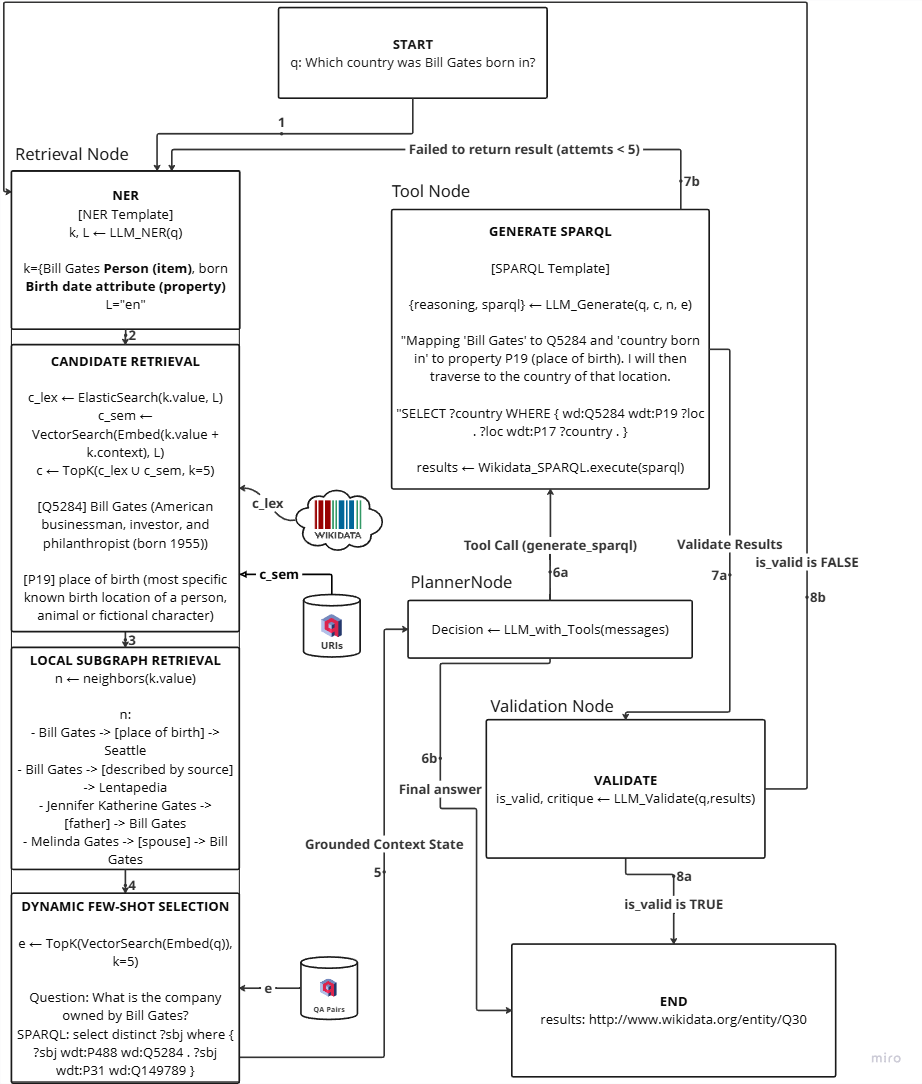
\includegraphics[width=\textwidth, trim=0 0 50 0, clip]{Miscellaneous/method.png} 
     \fbox{
    \parbox{0.95\textwidth}{
      \small
      \textbf{NER Template (Retrieval Node)} \\
      \textit{Your task is to extract all relevant keywords and phrases from the given question that could help in identifying Wikidata entities and properties. For each keyword, provide a 'context' description based on the question. You must also identify the language of the question. The question can be in any language.}
    }
  }
    
  \fbox{
    \parbox{0.95\textwidth}{
      \small
      \textbf{SPARQL Template (Tool Node)} \\
      \textit{You are an expert Wikidata SPARQL developer. Your goal is to construct a syntactically correct and semantically accurate SPARQL query to answer the user's question. 
      Context Data: [User Question],[Candidate Entities with local graph neighbors], [Few-Shot Examples].}
    }
  }
    \caption{The proposed agentic Text-to-SPARQL workflow.}
    \label{fig:system_architecture}
\end{figure}

The framework is formally governed by a dynamic state vector, denoted as $S$:
\begin{equation}
    S = \{q, k, L, c, n, e, sq, r, a\}
\end{equation}
where:
\begin{itemize}
    \item $q$ represents the original user question in natural language.
    \item $k$ represents the set of extracted keywords and contextual descriptions.
    \item $L$ denotes the detected language of the input question.
    \item $c$ represents the set of candidate entities retrieved from the knowledge graph.
    \item $n$ represents the local topological subgraph (1st-hop neighbors) of the candidates.
    \item $e$ denotes the dynamically retrieved few-shot semantic demonstrations.
    \item $sq$ is the generated SPARQL query hypothesis.
    \item $r$ is the execution result set returned by the target endpoint.
    \item $a$ is the iteration counter, tracking the number of refinement cycles.
     \item $M$ (\texttt{messages}): The core conversational memory. This is an append-only sequence of \texttt{BaseMessage} objects ($M = [m_1, m_2, \dots, m_t]$) that logs the agent's actions and environment feedback. Each message $m_i$ belongs to one of four rigid LangChain classes:
    \begin{itemize}
        \item \textbf{\texttt{HumanMessage}:} The initial input provided by the user.
        \item \textbf{\texttt{AIMessage}:} The outputs from the central reasoning engine, primarily comprising explicit tool calls containing the generated SPARQL query hypotheses.
        \item \textbf{\texttt{ToolMessage}:} The empirical observations returned by the external environment, including raw JSON result sets from the Wikidata endpoint or specific syntax error logs if execution fails.
        \item \textbf{\texttt{SystemMessage}:} Autonomous feedback, semantic critiques, and routing instructions injected into the state by the Validation Node to guide the LLM during self-correction loops.
    \end{itemize}
\end{itemize}

The query generation process flows through four interconnected nodes (Retrieval, Planning, Tool, and Validation), continuously updating this state vector until a valid, non-empty result set $r$ is achieved, or the maximum iteration threshold $a_{max}$ is reached.

\subsection{The Retrieval Node: Contextual Grounding}
\label{sec:retrieval_node}
The Retrieval Node serves as the foundational grounding layer of the framework. Its primary function is to transform the raw, ambiguous natural language question $q$ into a semantically enriched context, bridging the lexical gap~\cite{hoffner_survey_2017} between the user's intent and the knowledge graph's specific ontology. This process is decomposed into four sequential sub-tasks.

\subsubsection{Entity Recognition and Intent Extraction}
The workflow initiates with a multi-task extraction prompt designed to identify key semantic anchors within the question. The agent concurrently extracts key entities $k$ (including proper names, locations, and essential verbs) and detects the ISO language code $L$. 

To mitigate early-stage semantic ambiguity, the agent is instructed to generate a brief contextual description for each extracted keyword, clarifying its ontological role. For example, rather than simply extracting the keyword ``born,'' the agent tags it with a contextual footprint (e.g., ``Birth date attribute (Property)''). This enriched keyword-description pair is critical for the downstream retrieval process, ensuring that subsequent searches are grounded in the user's specific semantic intent rather than mere string similarity.

To enforce consistent behavior from the LLM during this stage, the system employs a specialized zero-shot prompt template. The prompt is designed to output structured JSON, ensuring the downstream RAG pipelines can programmatically parse the extracted arrays. 

\newpage

Listing~\ref{lst:ner_prompt} details the exact extraction instructions provided to the reasoning engine.

\begin{lstlisting}[basicstyle=\ttfamily\footnotesize, frame=single, caption={The zero-shot System Prompt utilized by the Retrieval Node for concurrent Named Entity Recognition (NER) and Language Detection, enforcing a strict JSON output schema.}, label={lst:ner_prompt}]
Your task is to extract all relevant keywords and phrases from the given
question that could help in identifying Wikidata entities and properties. 
For each keyword, provide a 'context' description based on the question. 
You must also identify the language of the question.
The question can be in any language. 

Question: 
{question}

Format:
- Format your response as a JSON object with the following keys:
    - "lang": A string representing the language code of the question 
    (e.g., "en", "es", "fr").
    - "keywords": A list of JSON objects. Each object must have these 
    three keys:
        - "value": The extracted keyword or phrase as a string.
        - "context": A short 3-5 word description of what this entity likely 
        represents in the context of the question 
        (e.g., "mathematical concept", "person", "city").
        - "type": The type of the keyword. Must be one of the following strings:
            - "item": For distinct entities like people, places, organizations,
            or concepts (e.g., "Leonardo da Vinci", "Paris", "Google", 
            "Mona Lisa").
            - "property": For attributes, relationships, or actions related 
            to an item (e.g., "date of birth", "capital of", "invented",
            "painted").
- If no relevant keywords are found, the "keywords" list should be an 
empty list [].
\end{lstlisting}

This explicit instruction forces the LLM to disambiguate terms preemptively, transforming a single ambiguous keyword into an enriched search anchor prior to querying the Qdrant index.

\subsubsection{Knowledge Graph Dump Processing and Index Construction}
\label{sec:dump_processing}

To enable the semantic retrieval pathway ($c_{sem}$) and the dynamic few-shot selection ($e$) without relying entirely on slow, external APIs, a critical prerequisite of our methodology was the construction of localized dense vector indices. This required processing a massive, offline Wikidata JSON dump. The raw Wikidata dump is highly nested and contains vast amounts of metadata (sitelinks, references, edit history) that are irrelevant for semantic embedding. 

The data preparation pipeline operated in three sequential stages:

\paragraph{1. Extraction and Filtering}
We parsed a recent Wikidata JSON dump. Because embedding the entirety of Wikidata's item space (over 100 million entities) is computationally prohibitive and largely unnecessary for schema mapping, the extraction focused on \textbf{standardizing the core ontology}. We extracted:
\begin{itemize}
   \item \textbf{All Item Identifiers (Q-nodes):} For example: \texttt{wd:Q123} (September), \texttt{wd:Q5284} (Bill Gates), ensuring that common targets for Named Entity Recognition (NER) were available in the local vector space.
    \item \textbf{All Property Identifiers (P-nodes):} For example, \texttt{wdt:P19} (place of birth) or \texttt{wdt:P31} (instance of).
\end{itemize}

Listing~\ref{lst:raw_wikidata} illustrates the sheer complexity of the raw JSON structure for a simple item, highlighting the necessity of the extraction phase.

\begin{lstlisting}[basicstyle=\ttfamily\footnotesize, frame=single, caption={Snippet of Raw Wikidata JSON structure (highly nested and verbose).}, label={lst:raw_wikidata}]
{
  "id": "Q123",
  "type": "item",
  "labels": {
    "en": { "language": "en", "value": "September" }
  },
  "descriptions": {
    "en": { "language": "en", "value": "ninth month of the year" }
  },
  "claims": {
    "P31": [ 
      {
        "mainsnak": { 
          "datavalue": { "value": { "id": "Q47018901" } } 
        }
      } 
    ]
  }
}
\end{lstlisting}

\paragraph{2. Semantic Concatenation}
To maximize the semantic density of the embedding, the nested JSON was flattened. For each extracted identifier (both P-nodes and Q-nodes), we aggregated its canonical English label, its aliases, and its descriptive text. These fields were concatenated using a special \texttt{[SEP]} separator token. This format ensures the embedding model captures the full semantic footprint of the entity in a single dense vector.

Listing~\ref{lst:processed_payload} demonstrates the output of this concatenation step, transforming the complex graph node into a dense, linguistically rich string.

\begin{lstlisting}[basicstyle=\ttfamily\footnotesize, frame=single, caption={Extracted and Concatenated Keyword Payload for Embedding.}, label={lst:processed_payload}]
{
  "id": "wdt:P19",
  "semantic_string": "place of birth [SEP] most specific known location where 
  a person was born"
},
{
  "id": "wd:Q123",
  "semantic_string": "September [SEP] ninth month of the year"
}
\end{lstlisting}

\paragraph{3. Embedding Model Selection and Benchmarking}
The concatenated textual representations required projection into a dense vector space. Because agentic workflows operate in continuous loops, the Retrieval Node may be invoked multiple times per user query. Consequently, the chosen embedding model had to balance three strictly competing constraints: \textbf{inference latency} (execution speed), \textbf{multilingual capacity}, and \textbf{retrieval performance} (accuracy).

To empirically determine the optimal encoder, we benchmarked five prominent models from the Massive Text Embedding Benchmark (MTEB)~\cite{mteb2024leaderboard} leaderboard. We measured the single-pass CPU inference latency (to simulate localized deployment) and compared it against the official MTEB retrieval performance scores. 

\begin{table}[htbp]
\centering
\caption{Performance vs. Efficiency Trade-off for Evaluated Embedding Models. MTEB scores represent the average retrieval performance across benchmarked datasets.}
\label{tab:model_performance}
\begin{tabular}{lccc}
\hline
\textbf{Model Name} & \textbf{Parameters} & \textbf{CPU Latency} & \textbf{MTEB Score (Avg)} \\
\hline
\texttt{all-MiniLM-L12-v2} & 33M & 3.1s & 56.53 (English) \\
\texttt{e5-small-v2} & 33M & 4.2s & 62.25 (English) \\
\texttt{multilingual-e5-small} & 118M & 3.2s & 61.30 (Multilingual) \\
\texttt{multilingual-e5-base} & 278M & 7.1s & 63.20 (Multilingual) \\
\texttt{multilingual-e5-large-instruct} & 568M & 0.1s\textsuperscript{*} & 64.41 (Multilingual) \\
\hline
\multicolumn{4}{l}{\footnotesize \textsuperscript{*} \textit{Note: Extrapolated GPU acceleration; CPU inference omitted due to memory constraints.}} \\
\end{tabular}
\end{table}

As illustrated in Table~\ref{tab:model_performance}, models like \texttt{multilingual-e5-base} (278M) and \texttt{large} (568M) offer slightly higher theoretical semantic representation (MTEB scores $>63$). However, their high CPU latency (e.g., 7.1 seconds for the base model) introduces severe bottlenecks into the cyclic agentic pipeline, where the retrieval node is called repeatedly. Conversely, while \texttt{all-MiniLM-L12-v2} executes rapidly, it fundamentally lacks the cross-lingual projection necessary for the multilingual QALD-10 evaluation.

Therefore, \texttt{intfloat/multilingual-e5-small} was selected as the optimal backbone. It sacrifices less than 3 points of MTEB accuracy compared to the largest models, while executing in a fraction of the time (3.2 seconds on CPU) and natively aligning multiple languages into the same vector space.

By pre-computing this semantic index offline, the system effectively bypasses the strict lexical limitations of standard Wikidata API endpoints at runtime, enabling the agent to perform purely conceptual searches (e.g., mapping the informal word "born" to the formal dense vector of \texttt{wdt:P19}).

 To ensure maximum coverage for entity resolution, the local Qdrant vector index embeds exactly \textbf{100\%} of Wikidata's core entity vocabulary—encompassing the multilingual \textit{fingerprints} (Labels, Aliases, and Descriptions) of all 121+ million Items and 11,000+ Properties. However, the system embeds exactly \textbf{0\%} of the underlying factual graph. The billions of Claims, Qualifiers, and Statements are intentionally excluded from the local vector space. 

By explicitly isolating the entity metadata from the structural graph, the semantic embeddings are strictly utilized for Schema and Entity Alignment. The system does not perform factual retrieval or graph traversal locally; all logical multi-hop traversals over Wikidata's complex reified Statements rely entirely on the live Wikidata SPARQL endpoint.

\subsubsection{Hybrid Candidate Retrieval}
\label{sec:hybrid_retrieval}
To maximize recall and effectively navigate the massive entity space of knowledge graphs like Wikidata, the system implements a hybrid candidate retrieval strategy. This strategy aggregates candidate entities $c$ from two complementary pathways: a lexical search ($c_{lex}$) and a semantic vector search ($c_{sem}$).

\paragraph{The Lexical Pathway ($c_{lex}$)} 
The system queries the standard search API (e.g., Wikidata ElasticSearch) using the extracted keywords $k$. By explicitly passing the detected language parameter $L$, the system restricts label and alias matching to the user's specific language, significantly reducing cross-lingual noise. 

However, pure lexical matching inherently suffers from homonym ambiguity. To resolve this (e.g., distinguishing between ``Bill Gates'' the person and ``Bill Gates'' the documentary), a semantic reranking layer is applied. As illustrated in Figure~\ref{fig:cosine_similarity_diagram}, a mathematical comparison is computed between the dense embedding of the user's intent (the keyword combined with the LLM-generated context) and the dense embedding of each candidate's canonical Wikidata description.

\textbf{Metric Selection (Cosine Similarity):} The choice of Cosine Similarity over alternative metrics like Euclidean distance ($L_2$) or raw Dot Product is deliberate. Euclidean distance is highly sensitive to vector magnitude, which inherently fluctuates based on the length of the input text. Because the inputs being compared are highly asymmetrical in length—a short user keyword phrase versus a lengthy, detailed Wikidata description—Euclidean distance would artificially penalize the match. Cosine similarity natively normalizes magnitude, isolating the angle between the vectors to focus purely on semantic "direction." Furthermore, the chosen encoder (\texttt{multilingual-e5-small}) was pre-trained using contrastive loss optimized specifically for cosine-based similarity search.

\textbf{Threshold Optimization (0.85):} Following the calculation, candidates falling below a strict similarity score of 0.85 are discarded. This specific hyperparameter was empirically derived to manage the LLM's context window. Setting the threshold too low (e.g., $<0.5$) allows "noise" into the pipeline, flooding the prompt with irrelevant homonyms (False Positives) which severely degrades LLM generation accuracy. Conversely, setting the threshold too high (e.g., $>0.85$) creates a strict semantic bottleneck (False Negatives), rejecting valid Wikidata entities simply because the user's natural language phrasing deviated slightly from Wikidata's formal ontology. A threshold of 0.85 optimally balances recall and precision, acting as a robust semantic filter.

\begin{figure}[H]
\centering
\begin{tikzpicture}[
    scale=0.8, transform shape, 
    node distance=0.8cm and 1.2cm, 
    base/.style={rectangle, draw=black, thick, align=center, inner sep=2mm, text=black},
    input/.style={base, rounded corners, fill=blue!10, text width=3.8cm, minimum height=0.8cm},
    process/.style={base, fill=green!10, text width=3.8cm, minimum height=0.8cm},
    vector/.style={base, dashed, fill=gray!10, text width=3.5cm, minimum height=0.6cm},
    math/.style={base, rounded corners, fill=orange!15, text width=3.2cm},
    output/.style={base, rounded corners, fill=green!20, text width=5cm, minimum height=0.8cm},
    arrow/.style={-{Stealth[scale=1]}, thick, draw=black}
]

\node (query) [input] {\textbf{User Intent}\\ \footnotesize "Which country was Bill Gates born in?"};
\node (candidate) [input, right=1.2cm of query] {\textbf{KG Candidate}\\ \footnotesize "Bill Gates [SEP] American businessman..."};

\node (embed1) [process, below=of query] {\textbf{Embedding Model}\\ \footnotesize (multilingual-e5-small)};
\node (embed2) [process, below=of candidate] {\textbf{Embedding Model}\\ \footnotesize (multilingual-e5-small)};

\node (vec1) [vector, below=of embed1] {\textbf{Vector $A$}\\ \footnotesize $[0.12, -0.45, \dots, 0.89]$};
\node (vec2) [vector, below=of embed2] {\textbf{Vector $B$}\\ \footnotesize $[0.14, -0.41, \dots, 0.92]$};

\node (cossim) [math] at ($(vec1)!0.5!(vec2) - (0, 1.4cm)$) {\textbf{Cosine Similarity}\\ \normalsize $\frac{A \cdot B}{||A|| ||B||}$};

\node (decision) [output, below=0.6cm of cossim] {\textbf{Score: 0.89}\\ \footnotesize ($0.85>$ Threshold) $\rightarrow$ \textbf{Accept}};

\draw [arrow] (query) -- (embed1);
\draw [arrow] (candidate) -- (embed2);
\draw [arrow] (embed1) -- (vec1);
\draw [arrow] (embed2) -- (vec2);
\draw [arrow] (vec1) |- (cossim);
\draw [arrow] (vec2) |- (cossim);
\draw [arrow] (cossim) -- (decision);

\draw [dashed, draw=gray, thick] 
    ($(embed1.north west)+(-0.3, 0.3)$) rectangle ($(vec2.south east)+(0.3, -0.3)$);
\node [text=gray] at ($(embed1.north west)+(1.2, 0.5)$) {\textit{Dense Semantic Space}};

\end{tikzpicture}
\caption{The Semantic Reranking Pipeline. Both the enriched user intent and the candidate's canonical Wikidata description are projected into a dense semantic space. Their cosine similarity is mathematically calculated to filter out lexically identical but semantically irrelevant homonyms.}
\label{fig:cosine_similarity_diagram}
\end{figure}

Table~\ref{tab:semantic_reranking} illustrates this disambiguation mechanism in action. While the standard API indiscriminately returns multiple exact string matches for "Bill Gates", the semantic reranker successfully filters the results based on the contextual intent.

\begin{table}[htbp]
\centering
\small 
\caption{Example of the Lexical Pathway's Semantic Reranking. The system uses the LLM-generated context to filter out exact-match homonyms based on Cosine Similarity.}
\label{tab:semantic_reranking}
\begin{tabular}{p{2cm} p{1.8cm} p{5.2cm} c c} 
\hline
\textbf{Wikidata ID} & \textbf{Label} & \textbf{Entity Description} & \textbf{Cosine Sim.} & \textbf{Action} \\
\hline
\multicolumn{5}{c}{\textbf{Extracted User Intent:} \textit{"Bill Gates" [SEP] Target Entity: Person}} \\
\hline
\texttt{wd:Q5284} & Bill Gates & American businessman, investor, and philanthropist & \textbf{0.89} & \textbf{Keep} \\
\texttt{wd:Q4909115} & Bill Gates & 2000 American documentary film directed by... & 0.42 & Discard \\
\texttt{wd:Q111460305}& Bill Gates & English footballer (born 1905) & \textbf{0.78} & \textbf{Keep} \\
\hline
\end{tabular}
\end{table}

By actively discarding low-similarity candidates like the documentary film (Cosine Sim: $0.42$), this targeted elimination successfully cleans the noise from the standard API output before the candidates are passed to the reasoning agent.

\paragraph{The Semantic Pathway ($c_{sem}$)} 
Concurrently, the system queries the pre-embedded Qdrant vector index to handle synonyms, complex phrasing, and lexical gaps~\cite{hoffner_survey_2017} that defeat standard text searches. Utilizing the highly efficient multilingual embedding model selected in Section~\ref{sec:dump_processing}, the user's keywords are projected into a shared semantic space alongside knowledge graph properties and items. This enables cross-lingual candidate retrieval, allowing a query in Chinese or German to map seamlessly to an English-labeled property based purely on conceptual proximity.

The final candidate set $c$ is defined as the union of the top-$k$ unique results from both pathways:
\begin{equation}
    c = TopK(c_{lex}) \cup TopK(c_{sem})
\end{equation}

\subsubsection{Local Subgraph Extraction (Topological Grounding)}
\label{sec:topological_grounding}
Relying solely on candidate labels and descriptions is often insufficient for resolving deep structural ambiguities. To provide the generative model with an accurate structural blueprint, the framework dynamically fetches the local graph neighborhood for each candidate in $c$. 

The system executes lightweight SPARQL queries directly against the Wikidata endpoint to extract the 1st-hop subgraph $n$, capturing both incoming and outgoing edges. To avoid saturating the LLM's context window with massive amounts of data (especially for highly connected "hub" entities), these queries extract the distinct predicates (properties) and a sample of their target objects, strictly limited to a small result set.

Using the disambiguated candidate for "Bill Gates" (\texttt{wd:Q5284}) as an example, the system generates and executes the following programmatic queries:

\paragraph{1. Outgoing Edges Retrieval}
The first query captures the relational pathways originating from the candidate entity ($Candidate \rightarrow Predicate \rightarrow Object$). This tells the LLM what properties the entity inherently possesses (e.g., place of birth, occupation, educated at).

\noindent 
\begin{minipage}{\textwidth}
\begin{lstlisting}[basicstyle=\ttfamily\footnotesize, frame=single, caption={SPARQL query dynamically generated by the Retrieval Node to fetch outgoing 1st-hop edges for wd:Q5284.}, label={lst:outgoing_edges}]
SELECT DISTINCT ?propLabel ?valLabel WHERE {
  wd:Q5284 ?p ?val .
  ?prop wikibase:directClaim ?p .
  ?prop rdfs:label ?propLabel .
  ?val rdfs:label ?valLabel .
  FILTER(LANG(?propLabel) = "en" && LANG(?valLabel) = "en")
} LIMIT 5
\end{lstlisting}
\end{minipage}

\paragraph{2. Incoming Edges Retrieval}
The second query captures pathways where the candidate entity is the target ($Subject \rightarrow Predicate \rightarrow Candidate$). This is critical for answering passive questions (e.g., "Who was founded by Bill Gates?").

\begin{lstlisting}[basicstyle=\ttfamily\footnotesize, frame=single, caption={SPARQL query to fetch incoming 1st-hop edges, where wd:Q5284 acts as the object.}, label={lst:incoming_edges}]
SELECT DISTINCT ?subjLabel ?propLabel WHERE {
  ?subj ?p wd:Q5284 .
  ?prop wikibase:directClaim ?p .
  ?prop rdfs:label ?propLabel .
  ?subj rdfs:label ?subjLabel .
  FILTER(LANG(?propLabel) = "en" && LANG(?subjLabel) = "en")
} LIMIT 5
\end{lstlisting}

\paragraph{Context Injection}
The JSON result sets returned by these two queries are parsed, stripped of redundant metadata, and concatenated into a compact topological blueprint. For example, the outgoing edges query reveals that \texttt{wd:Q5284} connects to "Seattle" via \texttt{wdt:P19} (place of birth). 

By injecting this exact structural context directly into the state vector $S$, the system grounds the LLM's reasoning in the actual ontology of the knowledge graph. This mechanism drastically reduces the hallucination of non-existent predicates (e.g., preventing the LLM from guessing a fake property like \texttt{wdt:bornIn}) and enables precise, context-aware query generation.

\subsubsection{Dynamic Few-Shot Selection (Syntax Grounding)}
\label{sec:dynamic_few_shot}

While Topological Grounding (Section~\ref{sec:topological_grounding}) ensures the LLM selects valid entities and predicates, it does not guarantee that the generated SPARQL \textit{syntax} will be structurally correct. SPARQL queries often require complex operators—such as aggregations (\texttt{GROUP BY}, \texttt{COUNT}), temporal filters (\texttt{FILTER(YEAR(?date) > 2000)}), or nested \texttt{OPTIONAL} clauses—that zero-shot LLMs frequently construct incorrectly. 

To guide the syntactic structure of the final query, the framework employs In-Context Learning (ICL) via \textbf{Dynamic Few-Shot Selection}. 

\paragraph{The Limitation of Static Prompting}
Traditional few-shot prompting relies on a static set of manually curated demonstrations embedded permanently in the system prompt. However, because the semantic structures of user questions are incredibly diverse, a static prompt containing 5 examples cannot possibly cover the thousands of potential SPARQL query topologies. Adding 50 examples to cover all topologies would instantly saturate the LLM's context window, increasing latency and API costs while decreasing reasoning performance (often referred to as the "lost in the middle" phenomenon~\cite{liu2024lost}).

\paragraph{Dynamic Retrieval from LC-QuAD 2.0}
To solve this, our framework dynamically retrieves only the most relevant syntactic demonstrations at runtime. To construct the demonstration index, we utilized the \textbf{LC-QuAD 2.0} dataset~\cite{dubey2019lcquad}, a large-scale Knowledge Graph Question Answering corpus containing 30,000 highly complex, verified (Question, SPARQL) pairs mapped to Wikidata.

During the offline data engineering phase, the natural language questions from LC-QuAD 2.0 were embedded into dense vectors using the \texttt{intfloat/multilingual-e5-small} encoder and stored in a dedicated Qdrant collection. 

\paragraph{Runtime Execution and Example Injection}
At runtime, the user's incoming question $q$ is encoded into the same vector space. The system performs an Approximate Nearest Neighbor (ANN) search using cosine similarity to retrieve the top-$k$ ($k=3$) most semantically and structurally similar question-query pairs $e$.

For example, if the user asks a question requiring a counting aggregation, the vector search will naturally pull a demonstration from the database that utilizes a \texttt{COUNT} operator, effectively teaching the LLM the correct syntax on the fly.

Listing~\ref{lst:few_shot_example} illustrates a formatted demonstration dynamically retrieved and injected into the LLM's context window.

\noindent
\begin{minipage}{\textwidth}
\begin{lstlisting}[basicstyle=\ttfamily\footnotesize, frame=single, caption={Example of a dynamically retrieved Few-Shot demonstration injected into the LLM prompt to teach aggregation syntax.}, label={lst:few_shot_example}]
[Demonstration 1]
User Question: "How many children does Bill Gates have?"
Reasoning: The user is asking for a quantitative count of entities connected via 
wdt:P40 (child). I must use a SELECT query with the COUNT() aggregation operator 
and group the results.
SPARQL Query: 
SELECT (COUNT(?child) AS ?count) WHERE { 
  wd:Q5284 wdt:P40 ?child . 
}
\end{lstlisting}
\end{minipage}

By injecting these dynamically retrieved, empirically verified examples $e$ into the state vector $S$, the generation model can adapt its syntax to specific query topologies without relying on static templates. This dual-grounding approach—combining Topological Grounding for vocabulary and Dynamic Few-Shot for syntax—forms the robust foundation of the framework's generation capabilities.

\subsection{Agentic Reasoning and Query Generation}
\label{sec:agentic_generation}

While the Retrieval Node successfully grounds candidate entities in their local topological structure and retrieves relevant syntax demonstrations, synthesizing this heterogeneous data into a syntactically valid SPARQL query requires dynamic reasoning. The framework employs an LLM operating as a central Planner and Tool executor, transitioning the methodology from static data retrieval to autonomous query formulation.

\subsubsection{The Central Reasoning Node (LLM Node): State Evaluation and Routing}
Rather than relying on a rigidly scripted sequence, the framework utilizes a central LLM node to orchestrate the control flow. This node acts as the system's "Planner," continuously evaluating the state vector $S$—which includes the user's question, the conversation history, and any existing execution results.

The central LLM utilizes native function-calling (tool-binding) capabilities to make a cognitive decision: \textit{Do I have enough empirical information to definitively answer the user's query, or do I need to invoke an external tool?} 

To facilitate this autonomous orchestration, the Central Reasoning Node is equipped with a strictly defined repertoire of tools:
\begin{itemize}
    \item \textbf{\texttt{generate\_sparql}:} The primary syntax tool. It commands the Tool Node to synthesize an executable SPARQL hypothesis based on the retrieved topological graph context and few-shot demonstrations.
    \item \textbf{\texttt{validate\_results}:} The diagnostic tool. It invokes the Validation Node to semantically verify if the returned Wikidata URIs structurally align with the expected answer type of the user's original question.
\end{itemize}

This decision-making process drives the \textbf{Conditional Routing} of the LangGraph architecture, managed by a dedicated routing function (\texttt{should\_continue}). This enables three distinct execution paths:
\begin{enumerate}
    \item \textbf{Initial Tool Invocation:} If the state is empty of SPARQL results, the LLM recognizes the information gap. It emits a tool call for \texttt{generate\_sparql}, and the routing function directs the state to the Tool Executor Node.
    \item \textbf{Error Handling and Re-Routing:} If the previous tool call resulted in a syntax error or returned no results, the routing function loops the state back. The LLM processes the error message as context and re-invokes the Tool Node to attempt a correction.
    \item \textbf{Final Answer Synthesis:} Once a valid result set is returned by the Wikidata endpoint and verified by the Validator Node, the state loops back to the LLM. The LLM determines that the tool-use condition is satisfied, synthesizes the raw JSON results into a natural language response using the \texttt{submit\_final\_answer} tool, and the routing function transitions the graph to the \texttt{END} state.
\end{enumerate}

By decoupling the high-level decision-making (the LLM Node) from the granular syntax execution (the Tool Node) and semantic verification (the Validation Node), the system prevents the language model from becoming overwhelmed by competing instructions.

\subsubsection{The Tool Node: Structured Generation and CoT}
Upon determining the execution strategy, the state transitions to the Tool Node. In traditional LLM applications, generative models frequently output conversational filler (e.g., "Here is the query you requested: ..."), which breaks automated execution pipelines. To enforce strict structural discipline, the Tool Node utilizes the LLM's structured output capabilities (e.g., JSON mode or tool calling) to mandate a rigid dual-field JSON schema.

Listing~\ref{lst:json_schema} illustrates the exact schema enforced by the system, ensuring programmatic determinism when parsing the LLM's response.

\begin{lstlisting}[basicstyle=\ttfamily\footnotesize, frame=single, caption={The mandated JSON schema enforced by the Tool Node to guarantee programmatic parsing of the generated query.}, label={lst:json_schema}]
{
  "reasoning_trace": "string (Explicit Chain-of-Thought deduction)",
  "sparql_query": "string (Syntactically valid and executable SPARQL)"
}
\end{lstlisting}

This dual-field structure forces the model into a two-step cognitive process:
\paragraph{1. The Reasoning Trace (Chain-of-Thought)}
Before generating any syntax, the model must explicitly articulate its logical deductions. It is prompted to justify its entity selection, predicate traversal, and aggregation logic (e.g., \textit{``Mapping 'Bill Gates' to \texttt{wd:Q5284} and traversing via \texttt{wdt:P19} for birthplace. A 1-hop SELECT query is sufficient.''}). This forced Chain-of-Thought (CoT) reasoning systematically mitigates common graph-traversal errors, such as subject-object inversions (``triple-flips''), by ensuring the model logically aligns the subject and predicate directions \textit{before} writing the code.

\paragraph{2. The SPARQL Hypothesis ($sq$)}
Following the reasoning trace, the node generates the executable SPARQL query. The syntax is dynamically formatted based on the question's intent, utilizing \texttt{SELECT} clauses for list extraction, \texttt{ASK} for boolean verification, or applying aggregations (\texttt{COUNT}, \texttt{ORDER BY}) as guided by the dynamically retrieved few-shot examples $e$.

\subsubsection{SPARQL Generation Prompt Design}
The generation prompt is the most critical interface in the agentic workflow. It acts as the synthesizer, injecting the massively heterogeneous RAG context directly into the LLM's working memory. To prevent schema hallucination, the system prompt rigidly defines the boundaries of the model's knowledge, instructing it to rely \textit{only} on the provided topological context.

Foundational LLMs inherently possess a vast amount of pre-trained knowledge regarding the Wikidata ontology. However, this parametric memory is often outdated, generalized, or structurally imprecise. When queried in an unconstrained manner, models frequently succumb to "parametric overconfidence"—hallucinating non-existent properties (e.g., guessing \texttt{wdt:bornIn} instead of \texttt{wdt:P19}). Therefore, the system prompt is engineered to suppress this behavior, enforcing a strict "closed-book" reasoning environment where the model must map the user's intent exclusively to the retrieved candidate IDs.

Furthermore, the prompt architecture is systematically divided into five distinct operational zones to guide the model's cognitive process. First, it establishes a clear persona (``expert Wikidata SPARQL developer'') to align the model's generation probabilities toward technical code output. Second, it dictates an explicit analysis strategy, forcing the model to categorize the expected answer type (boolean, list, aggregation) before writing syntax. Third, it injects deterministic syntactic constraints. By explicitly hardcoding standard Wikidata prefixes, the mandatory \texttt{wikibase:label} service, and default \texttt{LIMIT} clauses into the system rules, the framework significantly reduces token generation overhead and eliminates common formatting errors that would otherwise trigger endpoint execution failures.

The dynamic prompt is constructed at runtime by concatenating the dynamically retrieved state variables (the user's question, the local subgraph candidates, and the few-shot demonstrations) into this strict system message, as shown in Listing~\ref{lst:system_prompt}.

\begin{lstlisting}[basicstyle=\ttfamily\footnotesize, frame=single, caption={The dynamic System Prompt template utilized by the Tool Node to enforce topological adherence and inject RAG context.}, label={lst:system_prompt}]
You are an expert Wikidata SPARQL developer. Your goal is to construct 
a syntactically correct and semantically accurate SPARQL query to answer
the user's question.

### 1. Analysis Strategy
- **Entities**: Map the user's keywords to the provided 
**Candidate Entities** (QIDs/PIDs).
- **Logic**: Determine if the user wants a list, a count, a specific date,
or a boolean (ASK) answer.

### 2. Constraints & Rules
- **Prefixes**: Assume standard prefixes (`wd:`, `wdt:`, `p:`, `ps:`, `pq:`)
are already defined. Do not output `PREFIX` lines.
- **Label Service**: If the user asks for names, always include: 
`SERVICE wikibase:label { bd:serviceParam wikibase:language "[AUTO_LANGUAGE],en". }`
- **Filtering**: Use `FILTER` for dates or string matching if necessary.
- **Limit**: Use `LIMIT 10` unless the user asks for "all" or a specific count.

### 3. Context Data
**User Question:** "{question}"

**Candidate Entities (Use these IDs):**
{candidates}

### 4. Few-Shot Examples
{examples}

### 5. Final Output
Return a **JSON object** with two keys:
1. "reasoning": A brief sentence explaining which entities and properties 
you chose.
2. "sparql": The valid SPARQL query string.
\end{lstlisting}

By explicitly feeding the \texttt{[Candidate Entities \& Local Graph Neighbors]} directly into the prompt template, the system bridges the gap between the LLM's vast but unreliable parametric memory and the actual structural reality of the Wikidata endpoint at runtime.

\subsubsection{Prompt Engineering for Autonomous Recovery}
To ensure the LLM correctly interprets the execution feedback and does not fall into infinite loops of repeating the same incorrect queries, the framework relies on highly structured, dynamic prompt templates injected during the routing phase.

\paragraph{Handling Empty Result Sets}
When a query executes without syntax errors but returns an empty result set ($r = \emptyset$), the system diagnoses a logical traversal error (e.g., overly restrictive filtering or an incorrect property path). To facilitate correction, the Tool Node constructs a dynamic critique prompt. 

Crucially, as shown in Listing~\ref{lst:failure_prompt}, the system tracks and injects the \texttt{\{previous\_queries\}} history. This prevents the agent from entering a deterministic loop where it repeatedly guesses the exact same incorrect graph pattern.

\begin{lstlisting}[basicstyle=\ttfamily\footnotesize, frame=single, caption={The dynamic feedback prompt injected into the state when a query returns no results, forcing the LLM to critique its previous attempts.}, label={lst:failure_prompt}]
The previous SPARQL query for the user task "{user_task}" returned no results.

Failed query:
{failed_query}

**Critique the failed query and suggest a correction.**

Here are the previously generated queries:
{previous_queries}

Try to modify and improve your next query to retrieve meaningful results.
\end{lstlisting}

\paragraph{The Semantic Evaluator Prompt}
If a query successfully returns a populated result set, the Validation Node executes a proactive semantic check before presenting the answer to the user. Because SPARQL queries typically return raw Wikidata URIs (e.g., \texttt{wd:Q73}), the system first utilizes the Wikidata API to fetch the human-readable labels and descriptions for the retrieved IDs. 

This enriched context is then passed to a dedicated LLM evaluation prompt, detailed in Listing~\ref{lst:validation_prompt}.

\begin{lstlisting}[basicstyle=\ttfamily\footnotesize, frame=single, caption={The strict evaluation prompt used by the Validation Node to ensure the retrieved entity types align with the user's semantic intent.}, label={lst:validation_prompt}]
You are an expert at validating SPARQL query results. 

User Question: "{question}"

SPARQL Query Results and Entity Context:
{results}

**Instructions:**
1. Check if the **Format** is correct (e.g., if the user asked for a list, 
is it a list?).
2. Check if the **Entity Types** make sense (e.g., if asked for a person, are the 
results people?). Use the provided 'Entity Definitions' to understand what the IDs 
represent.
3. Do NOT reject the result just because you don't know the specific fact, provided
the Entity Type is correct.

Does the result answer the question?
\end{lstlisting}

The third instruction in this prompt is a critical architectural decision. LLMs often suffer from "parametric overconfidence"—if the knowledge graph returns a highly obscure fact that contradicts the LLM's pre-trained memory, the LLM might incorrectly reject the valid graph result. By explicitly instructing the model to evaluate the \textit{Entity Type} rather than the \textit{Fact Validity}, the system successfully separates structural evaluation from factual hallucination, ensuring that obscure but structurally correct knowledge graph data is preserved and returned to the user.

\subsubsection{Query Execution and Endpoint Interfacing}
Immediately following generation, the Tool Node parses the JSON object, extracts the \texttt{sparql\_query} string, and autonomously executes the hypothesis against the target public Wikidata endpoint via an HTTP request. 

The raw JSON payload returned by the endpoint (or the HTTP error code if the query was structurally invalid or timed out) is captured and assigned to the result state variable $r$. This result, alongside the query itself, is then appended to the state vector and passed to the Validation layer to determine if the agentic loop should terminate or self-correct.

\subsection{Execution-Guided Semantic Validation}
\label{sec:validation_node}

A critical advancement in this architecture is the Validation Node, which introduces an iterative, execution-guided self-correction loop. Traditional Seq2Seq pipelines terminate upon receiving an empty result set or a syntax error. In contrast, our agentic framework treats these execution failures as deterministic feedback signals, enabling autonomous refinement.

Algorithm~\ref{alg:agentic_workflow} presents the complete cyclical generation and validation procedure.

\begin{algorithm}[H]
\caption{Cyclic Agentic Text-to-SPARQL Workflow (LangGraph)}
\label{alg:agentic_workflow}
\begin{algorithmic}[1]
\Require Natural language question $q$, max attempts $a_{max} = 5$
\Ensure Valid SPARQL query $sq$, Result set $r$
\State Initialize state vector $S \gets \{q\}$, attempts $a \gets 0$

\While{$a < a_{max}$}
    \State \textbf{Phase 1 - Contextual Grounding (retriever\_node):}
    \If{$a \geq 2$ or $S.candidates$ is empty} \Comment{Force Refresh Logic}
        \State $k, L \gets$ \text{get\_ner\_result}($q$)
        \State $c \gets$ \text{get\_candidates}($k, L$)
        \State $n \gets$ \text{enrich\_candidates}($c$) \Comment{Extract 1st-hop subgraphs}
        \State $e \gets$ \text{fetch\_similar\_qa\_pairs}($q, L$)
        \State Update $S \gets S \cup \{k, L, c, n, e\}$
    \EndIf

    \State \textbf{Phase 2 - Routing (llm\_node):}
    \State ToolCalls $\gets$ \text{LLM.bind\_tools}($S$)
    \If{ToolCalls is empty}
        \State \textbf{break} \Comment{No tools needed, output final answer}
    \EndIf
    
    \State \textbf{Phase 3 - Execution (tool\_node):}
    \State $a \gets a + 1$
    \State $r, error \gets$ \text{generate\_sparql}(ToolCalls)
    
    \If{$error \neq \text{Null}$ \textbf{or} $r = \emptyset$} 
        \State Append Failure Message to $S$
        \State \textbf{continue} \Comment{Loop back to retriever/llm to fix syntax}
    \EndIf
    
    \State \textbf{Phase 4 - Semantic Check (validation\_node):}
    \State QIDs $\gets$ \text{extract\_all\_qids}($r$)
    \State Labels $\gets$ \text{get\_wikidata\_labels}(QIDs)
    \State $is\_valid \gets$ \text{validate\_results}($q, r, Labels$)
    
    \If{\textbf{not} $is\_valid$}
        \State Append "Validator Feedback: Invalid" to $S$
        \State \textbf{continue} \Comment{Loop back and trigger force\_refresh}
    \EndIf
    
    \State \textbf{break} \Comment{Query executed successfully and passed validation}
\EndWhile

\Return $sq, r$
\end{algorithmic}
\end{algorithm}

As detailed in the algorithm, the Validation Node categorizes feedback into three distinct failure modes:

\begin{enumerate}
    \item \textbf{Syntax/Execution Errors:} If the endpoint rejects the query (e.g., missing prefixes, unmatched braces), the exact error message is appended to the prompt history. The LLM directly corrects the syntax in the next iteration.
    \item \textbf{Empty Result Sets:} If the query executes but returns nothing, the system diagnoses a logical error (e.g., traversing a relation in the wrong direction or applying an overly restrictive \texttt{FILTER}). The LLM is prompted to relax constraints or try an alternative predicate.
    \item \textbf{Semantic Invalidity:} If the query returns raw Wikidata identifiers, the Validation Node performs a proactive semantic check. It fetches human-readable labels for the retrieved IDs and utilizes a lightweight LLM evaluator to verify alignment with the user's intent. If a user asks for a ``person'' but the query returns a ``date,'' the system actively rejects the successful query, forces a retrieval refresh, and loops back.
\end{enumerate}

This autonomous recovery mechanism drastically reduces schema hallucinations and significantly boosts overall precision, terminating only when a valid result is found or the strict iteration cap ($a_{max} = 5$) is reached to prevent infinite loops.

\subsection{Implementation Details}
\label{sec:implementation_details}

The agentic framework is implemented in Python, utilizing the \textbf{LangGraph} library to construct the asynchronous cyclic state machine. The system's state is managed via LangGraph's \texttt{StateGraph} with strict \texttt{TypedDict} schemas to ensure reliable data passing between nodes.

The central reasoning, planning, and generation components were evaluated using two distinct foundational LLMs to assess both proprietary and open-weight capabilities:
\begin{itemize}
    \item \textbf{gpt-4.1-mini} (OpenAI): Utilized for its advanced function-calling reliability and superior multilingual reasoning capabilities.
    \item \textbf{nemotron-3-nano-30b} (NVIDIA): An efficiently scaled, open-weight model deployed to evaluate the framework's viability in localized, privacy-preserving environments.
\end{itemize}
For the Retrieval Node, dense semantic vector matching and dynamic few-shot example selection were powered by \textbf{Qdrant}, a high-performance local vector database. The multilingual embedding model \texttt{intfloat/multilingual-e5-small} was selected from the MTEB leaderboard for its low inference latency and robust cross-lingual projection. Lexical matching and local subgraph extraction were executed against the standard Wikidata ElasticSearch API and SPARQL endpoint. 

The agent was configured with a temperature of $0.0$ for all query generation and planning steps to maximize deterministic syntax adherence, while the iteration threshold was strictly capped at $5$ attempts per query to balance autonomous self-correction with system latency.

\subsection{Advantages and Limitations}
\label{sec:methodology_limitations}

The proposed agentic architecture introduces several distinct advantages over traditional sequence-to-sequence pipelines and static LLM prompting methods:

\begin{itemize}
    \item \textbf{Domain Agnosticism and Zero-Shot Transfer:} By relying on dynamic Retrieval-Augmented Generation (RAG) rather than static fine-tuning, the system can generalize to previously unseen graph structures. It discovers the schema at runtime, completely eliminating the need for expensive, domain-specific dataset curation and model retraining.
    \item \textbf{Autonomous Recovery and Resilience:} The execution-guided feedback loop allows the system to repair its own logical and syntactic errors. This provides a level of execution resilience entirely absent in standard NMT models, which fail silently upon generating a single incorrect token.
    \item \textbf{High Explainability and Auditability:} The mandated JSON schema enforces a Chain-of-Thought reasoning trace. This ensures that every generated query is accompanied by a human-readable justification of the entity selection and traversal logic, vastly simplifying error analysis and system debugging.
    \item \textbf{Modular and Extensible Architecture:} Because the framework is built using an asynchronous state machine (LangGraph), the components are strictly decoupled. The LLM reasoning backbone, the vector database (Qdrant), and the semantic checker can be independently upgraded or swapped (e.g., replacing GPT-4 with a local open-weight model) without altering the core routing logic.
    \item \textbf{Native Multilingual Support:} Traditional pipelines require distinct linguistic parsers for different languages. By synergizing a multilingual embedding model (\texttt{multilingual-e5-small}) with the inherent cross-lingual capabilities of foundational LLMs, the system processes queries in English, German, Russian, and Chinese through a unified, language-agnostic pipeline.
\end{itemize}

However, the agentic approach introduces inherent engineering and theoretical trade-offs that constrain its applicability:

\begin{itemize}
    \item \textbf{Inference Latency:} Cyclical graph execution incurs significantly higher latency than single-pass models. Resolving a complex query via 3 to 4 refinement loops—each requiring a network call to the LLM API, the vector database, and the SPARQL endpoint—may take several seconds. This makes the architecture unsuitable for systems requiring instantaneous, sub-100ms responses (e.g., real-time autocomplete search).
    \item \textbf{Context Window Saturation:} The system's reliance on topological grounding introduces vulnerabilities when processing "hub" entities. Highly connected nodes (e.g., "United States") possess tens of thousands of edges. Injecting these into the prompt necessitates strict truncation (e.g., \texttt{LIMIT 5}), which may inadvertently hide the correct predicate from the LLM, forcing a hallucination.
    \item \textbf{Endpoint Dependency and Volatility:} The self-correction loop relies entirely on the uptime and response time of the external Wikidata SPARQL endpoint. Network timeouts, rate-limiting, or server-side execution limits directly degrade the agent's ability to evaluate its hypotheses, often leading to terminal failures that are unrelated to the model's reasoning capabilities.
    \item \textbf{Cascading Error Propagation:} While the Validation Node can catch syntax and semantic errors, it cannot recover from catastrophic failures at the very beginning of the pipeline. If the Retrieval Node extracts the completely wrong keyword, or the Qdrant vector search retrieves entirely irrelevant P-nodes, the generation model is forced to reason over corrupted data. The LLM will confidently generate a query using the wrong topology, which the self-correction loop cannot fix.
\end{itemize}

\subsection{System Walkthrough and Running Examples}
\label{sec:system_walkthrough}
To concretely illustrate the architectural capabilities of the system—particularly the Topological Grounding and the Execution-Guided Validation loop defined in Algorithm~\ref{alg:agentic_workflow}—this section presents a step-by-step trace of the state vector ($S$) during execution.

\subsubsection{Case Study 1: Multi-Hop Reasoning with Topological Grounding}
A primary challenge in KGQA is translating a single natural language sentence into a multi-hop graph traversal. Traditional systems frequently fail when a conceptual relationship in language (e.g., "born in [Country]") does not directly map to a single edge in the knowledge graph. 

\textbf{User Query ($q$):} \textit{"Which country was Bill Gates born in?"}

\textbf{State Transition 1: Retrieval Node (NER \& Intent Extraction)}
The system initiates by passing $q$ to the multi-task extraction prompt. The LLM generates the following structured JSON, strictly adhering to the schema defined in Listing~\ref{lst:ner_prompt}. This step effectively disambiguates the semantic anchors before any database search occurs:

\noindent
\begin{minipage}{\textwidth}
\begin{lstlisting}[basicstyle=\ttfamily\footnotesize, frame=single, caption={NER and Intent Extraction Output. The LLM successfully categorizes the keywords into items and properties as dictated by the prompt.}, label={lst:ner_output}]
{
  "lang": "en",
  "keywords": [
    {
      "value": "Bill Gates",
      "context": "Target Entity: Person",
      "type": "item"
    },
    {
      "value": "born in",
      "context": "Relational constraint: Birth location",
      "type": "property"
    },
    {
      "value": "country",
      "context": "Expected Answer Type: Sovereign state",
      "type": "item"
    }
  ]
}
\end{lstlisting}
\end{minipage}

\textbf{State Transition 2: Topological Graph Injection}
Using the extracted keywords, the Hybrid Retrieval module queries the localized Qdrant index and the Wikidata API. It successfully links "Bill Gates" to \texttt{wd:Q5284}. Crucially, rather than guessing the property for "born in", the system retrieves the 1st-hop local subgraph for \texttt{wd:Q5284}. The injected context reveals that \texttt{wd:Q5284} does \textit{not} have a direct \texttt{wdt:P17} (country) property. Instead, it has a \texttt{wdt:P19} (place of birth) pointing to \texttt{wd:Q79} (Seattle), which in turn has a \texttt{wdt:P17} property pointing to \texttt{wd:Q30} (United States).

\textbf{State Transition 3: Planner and Tool Node (Generation)}
Armed with the topological blueprint, the Planner maps the user's intent to the available graph edges. The Tool Node generates the formal Reasoning Trace and the corresponding SPARQL query:

\noindent
\begin{minipage}{\textwidth}
\begin{lstlisting}[basicstyle=\ttfamily\footnotesize, frame=single, caption={Tool Node Query Generation}, label={lst:tool_gen}]
{
  "reasoning_trace": "The user asks for the country of birth for Bill Gates 
  (wd:Q5284). The local subgraph shows no direct 'country' edge from the person. 
  However, wd:Q5284 connects to wd:Q79 (Seattle) via wdt:P19 (place of birth).
  To find the country, I must perform a 2-hop traversal from the birth city 
  using wdt:P17 (country).",
  "sparql_query": "SELECT ?country WHERE 
  { wd:Q5284 wdt:P19 ?city . ?city wdt:P17 ?country . }"
}
\end{lstlisting}
\end{minipage}

The query executes successfully on the first iteration, returning \texttt{wd:Q30}, completely bypassing the structural hallucination that plagues zero-shot NMT models.

\subsubsection{Case Study 2: Autonomous Semantic Self-Correction}
The defining feature of this agentic framework is its ability to recover from logical errors using endpoint feedback. This case study demonstrates the \textbf{Semantic Check} mechanism defined in the Validation Node (Algorithm~\ref{alg:agentic_workflow}), where a query executes without syntax errors but violates the user's semantic intent based on the rules defined in the \texttt{validation\_prompt}.

\textbf{User Query ($q$):} \textit{"When was Albert Einstein born?"}

\textbf{Iteration 1: The Logical Error}
The Retrieval Node identifies "Albert Einstein" (\texttt{wd:Q937}) and the keyword "born". The Tool Node hypothesizes the following query:

\noindent
\begin{minipage}{\textwidth}
\begin{lstlisting}[basicstyle=\ttfamily\footnotesize, frame=single, caption={Iteration 1: Incorrect Property Selection}, label={lst:iteration_1}]
SELECT ?date WHERE { wd:Q937 wdt:P19 ?date . }
\end{lstlisting}
\end{minipage}

The query contains no syntax errors and executes successfully against the Wikidata endpoint. It returns the result \texttt{wd:Q73}. In a traditional Seq2Seq pipeline, the system would output this result to the user and terminate. 

\textbf{Iteration 2: The Validation Node Intervention}
Before returning the result, the Validation Node performs a proactive semantic evaluation. It extracts the raw QID (\texttt{wd:Q73}) and queries the Wikidata API for its human-readable label and description, discovering that it is "Ulm (city in Baden-Württemberg, Germany)". 

This enriched context is passed to the LLM Evaluator using the system's \texttt{validation\_prompt}. Following Instruction \#2 of the prompt (\textit{"Check if the Entity Types make sense"}), the Evaluator compares the retrieved type ("city") against the original intent ("When" $\rightarrow$ Expected Type: Date/Time). 

The Evaluator flags a critical semantic mismatch, outputs "Invalid", and the Validation Node dynamically generates the following text-based \texttt{SystemMessage}, appending it to the state history and incrementing the iteration counter ($a=1$):

\noindent
\begin{minipage}{\textwidth}
\begin{lstlisting}[basicstyle=\ttfamily\footnotesize, frame=single, caption={Actual SystemMessage injected into the LangGraph state by the Validation Node, forcing the LLM to correct the semantic mismatch.}, label={lst:validation_feedback}]
The previous query returned results, but the automated validator determined
they do not correctly answer the question: 'When was Albert Einstein born?'.
Validator Feedback: Invalid. The user asked 'When' indicating a date is required, 
but the query returned a geographic city ('Ulm').
Please analyze the previous query and results, and generate a 
CORRECTED SPARQL query.
\end{lstlisting}
\end{minipage}

\textbf{Iteration 3: The Correction}
The state loops back to the central LLM Node, appending this error feedback directly into the context window. The agent re-evaluates the topological subgraph for \texttt{wd:Q937}, specifically scanning for temporal predicates to satisfy the validator's critique. It identifies \texttt{wdt:P569} (date of birth) and generates the corrected query:

\noindent
\begin{minipage}{\textwidth}
\begin{lstlisting}[basicstyle=\ttfamily\footnotesize, frame=single, caption={Iteration 2: Corrected Query}, label={lst:corrected_query}]
SELECT ?date WHERE { wd:Q937 wdt:P569 ?date . }
\end{lstlisting}
\end{minipage}

This successfully returns the literal value \texttt{"1879-03-14"\^{}\^{}xsd:dateTime}, satisfying the semantic check and terminating the loop. This trace empirically proves the necessity of execution-guided agentic architectures; without the ability to "see" the endpoint's output and evaluate the entity types, the system would have confidently returned a city instead of a date.